\documentclass{beamer}
\usepackage{beamerthemesplit}
\usepackage{graphicx,url}
\usepackage[brazil]{babel}
\usepackage[utf8]{inputenc}

\mode<presentation>
{
  \usetheme{Ilmenau}
  \setbeamercovered{transparent}
}

\newcommand{\eng}[1]{\textit{#1}}
\newcommand{\obra}{\textit{Em torno da romã}}

\title{\obra{}: aplicações de operações de contorno na composição}
\author{Marcos da Silva Sampaio}
\date{28 de novembro de 2008}

\logo{\includegraphics[scale=.15]{logo-genos}}

\begin{document}

\frame{\titlepage}

\section{Introdução}

\frame{
  \frametitle{O que são contornos?}
  \begin{columns}[t]
    \column{8cm}
    \begin{enumerate}
    \item Perfis, desenhos ou formatos de objetos.
    \item Podem ser bidimensionais
    \item Podem associar:
      \begin{enumerate}
      \item altura a comprimento
      \item altura a largura
      \item altura a tempo
      \end{enumerate}
    \end{enumerate}

    \column[T]{3cm}
    \includegraphics[scale=.3]{roma-pura}
    
    \includegraphics[scale=.3]{contorno-com-roma}
  \end{columns}
}

\frame{
  \frametitle{Contornos em música}
  \begin{enumerate}
  \item Podem ser associados a altura, densidade, ritmo, homogeneidade
    de timbre, intensidade, etc.
  \item Contornos melódicos: movimentos de altura no tempo.
  \end{enumerate}
  \includegraphics{c-0312}
}

\frame{
  \frametitle{Por que contornos são importantes}
  \begin{enumerate}
  \item Podem ajudar a dar coerência a uma obra musical.
  \item Representam estruturas manipuláveis através de operações como
    inversão e retrogradação.
  \end{enumerate}
}

\frame{
  \frametitle{Justificativa para este trabalho}
  Apesar da possível coerência musical proporcionada por contornos e
  das operações disponíveis, são escassos estudos do uso sistemático
  de operações de contornos e suas combinações na composição musical.
}

\frame{
  \frametitle{Objetivo principal deste trabalho}
  Composição de uma obra musical com base em combinações de operações
  de contornos e a produção de seu memorial.
}

\frame{
  \frametitle{Objetivos secundários deste trabalho}
  \begin{enumerate}
  \item Desenvolvimento de um programa de computador para
    processamento de operações de contornos melódicos.
  \item Mapeamento de contornos para elementos musicais/composicionais.
  \item Levantamento do estado de arte de contornos melódicos.
  \end{enumerate}
}

\frame{
  \frametitle{Metodologia de trabalho}
  \begin{enumerate}
  \item Revisão de literatura.
  \item Mapeamento de contornos para elementos musicais.
  \item Composição de estudos para experimentação de possibilidades
    com contornos.
  \item Desenvolvimento de programa de computador para processamento
    de contornos.
  \item Composição da obra \obra{}.
  \end{enumerate}
}

\section{Contornos}

\subsection{Definições de contornos melódicos}

\frame{
  \frametitle{Definição 1}

  Movimento ascendente ou descendente entre notas adjacentes de uma
  melodia
  \cite{piston59:harmony,toch77:shaping,edworthy85:musical,dewitt.ea86:recognition}.

  \begin{figure}
    \centering
    \includegraphics[scale=.5]{5a-sinfonia}
    \caption{Fragmento da 5ª Sinfonia de Beethoven}
  \end{figure}

  \begin{itemize}
  \item Representação simbólica: (- + -)
  \end{itemize}
}

\frame{
  \frametitle{Definição 2}
  Conjunto ordenado de elementos distintos com ou sem repetição,
  numerados de forma ascendente \cite{morris93:directions}.

  \begin{figure}
    \centering
    \includegraphics[scale=.5]{5a-sinfonia}
    \caption{Fragmento da 5ª Sinfonia de Beethoven}
  \end{figure}

  \begin{itemize}
  \item Representação simbólica: (3 1 2 0)
  \end{itemize}
}

\frame{
  \frametitle{Comparação entre definições}

  \begin{figure}
    \centering
    \includegraphics[scale=.5]{5a-sinfonia}
    \caption{Fragmento da 5ª Sinfonia de Beethoven}
  \end{figure}

  \begin{columns}[t]
    \column{6cm}
    \begin{figure}
      \centering
      \includegraphics[scale=.5]{c-1010}
      \caption{Movimento ascendente/descendente entre alturas adjacentes}
    \end{figure}

    \column[T]{6cm}
    \begin{figure}
      \centering
      \includegraphics[scale=.5]{c-3120}
      \caption{Conjunto ordenado de elementos numerados}
    \end{figure}
  \end{columns}
}

\frame{
  \frametitle{Vantagens da definição de Morris}
  \begin{enumerate}
  \item Considera elementos não adjacentes de uma melodia.
  \item Expansível para outros elementos musicais além de altura, como
    densidade de acordes ou dinâmica.
  \end{enumerate}

  \includegraphics[scale=.5]{chord-densities-in-time}
  \hspace{2em}
  \includegraphics[scale=.5]{dynamics-in-time}
  \hspace{2em}
  \includegraphics[scale=.5]{c-1023}
}

\subsection{Outras considerações}

\frame{
  \frametitle{Outras considerações sobre este trabalho}
  \begin{enumerate}
  \item Não trabalhei com medida do tempo no contorno
  \item Definição de ``operações de contorno''
  \item Análises de obras a partir da perspectiva de contornos:
    Schoenberg \cite{friedmann85:methodology}, Webern
    \cite{clifford95:contour,sampaio08:analise}, Dallapicolla
    \cite{marvin88:generalized} e Mozart \cite{beard03:contour}.
  \end{enumerate}
}

\frame{
  \frametitle{Contornos em Etnomusicologia, Computação Musical e Percepção}
  \begin{enumerate}
  \item Etnomusicologia: Contornos para classificação de melodias
    \cite{adams76:melodic}.
  \item Computação musical: Contornos em sistemas \eng{query by
      humming} \cite{ghias.ea95:query}.
  \item Percepção: Semelhança entre contornos x semelhança entre
    alturas
    \cite{marvin88:generalized,friedmann90:ear,dowling.ea86:music,dowling.ea71:contour}.
  \end{enumerate}
}

\frame{
  \frametitle{Contorno como determinante composicional}
}

\subsection{Teorias de contornos}

\frame{
  \frametitle{Conceitos e operações de contornos}
  \begin{enumerate}
  \item Operações de mapeamento e comparação
    \cite{friedmann85:methodology,friedmann87:response,morris87:composition,morris93:directions,marvin.ea87:relating,clifford95:contour,polansky.ea92:possible,quinn97:fuzzy,beard03:contour}.
  \item Melodias com semelhança reconhecível apenas pelo contorno
    \includegraphics[scale=.7]{ly-0312}
    \includegraphics[scale=.6]{c-0312}
  \end{enumerate}

}

\frame{
  \frametitle{Representações de contornos}
  \begin{columns}[t]

    \column{6cm}
  \begin{enumerate}
  \item Representação simbólica
    \begin{itemize}
    \item Contorno: Z(2 0 3 1)
    \item Elementos: Z$_0=2$, Z$_1=0$, Z$_2=3$ e Z$_3=1$
    \end{itemize}
  \item Representação gráfica

    \includegraphics[scale=.6]{c-2031}
  \end{enumerate}

    \column[T]{4cm}
  \includegraphics[scale=.5]{ly-2031}
  \end{columns}
}

\frame{
  \frametitle{Representação de operações}
  \begin{itemize}
  \item Retrógrado de X(1 2 3): $retr(X(1\:2\:3))=Y(3\:2\:1)$
  \item Transposição de X(1 2 3) com fator 2: $transp(X(1\:2\:3)\:2)=W(3\:4\:5)$
  \item Concatenação de operações: $transp(retr(inv(rot(X(1\;2\;3))\;2))\;3)$
  \end{itemize}
}

\frame {
  \frametitle{Espaço de contorno}
  \begin{itemize}
  \item Elementos organizados do valor mais baixo para o mais alto,
    desconsiderando seus valores exatos.
  \item Contém segmentos e subconjuntos de segmentos de contornos.
  \end{itemize}
  \begin{figure}
    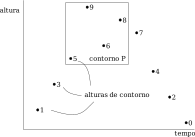
\includegraphics[scale=.8]{cspace-5968}
  \end{figure}
}

\frame {
  \frametitle{Exemplos de espaço de contorno}
  \begin{figure}
    \includegraphics[scale=.7]{cspace-564}
  \end{figure}
  \begin{figure}
    \includegraphics[scale=.7]{cspace-7420}
  \end{figure}
}

\frame{
  \frametitle{}
}

\section{Análise da obra}

\frame{
  \frametitle{}
}

\section{Conclusões}

\frame{
  \frametitle{}
}

\frame[allowframebreaks]{
  \frametitle{Referências}
  \bibliographystyle{alpha}
  \bibliography{melodic-contour,music-perception,composition,music-harmony-and-theory,programs,music-analysis,audio,genos,computer-science}
}

\end{document}
